%% ============================================================
%%  Nakuja N4 Recovery System – Continuous Assessment Presentation
%%  Beamer, metropolis theme
%% ============================================================
\documentclass[aspectratio=169, 11pt]{beamer}

\usetheme{metropolis}
\usepackage{graphicx}
\usepackage{booktabs}
\usepackage{xcolor}
\usepackage{amsmath}
\usepackage{tikz}
\usetikzlibrary{shapes.geometric, arrows.meta, positioning, calc}
\usepackage{grffile}   % handles spaces in filenames

% ---- colour palette ----
\definecolor{nakujaBlue}{RGB}{0,51,102}
\definecolor{nakujaOrange}{RGB}{220,100,0}
\definecolor{lightgray}{RGB}{240,240,240}

\setbeamercolor{frametitle}{bg=nakujaBlue, fg=white}
\setbeamercolor{progress bar}{fg=nakujaOrange}
\setbeamercolor{alerted text}{fg=nakujaOrange}
\setbeamercolor{block title}{bg=nakujaBlue!15, fg=nakujaBlue}
\setbeamercolor{block body}{bg=nakujaBlue!5}

\metroset{sectionpage=none, subsectionpage=none, progressbar=frametitle}

\graphicspath{{images/}{images/mechanical/}}

% ---- title info ----
\title{N4 Rocket Recovery System}
\subtitle{Continuous Assessment Presentation}
\author{Glenn Omondi}
\institute{Nakuja Project --- Final Year Project}
\date{March 2026}

%% ============================================================
\begin{document}

% ------------------------------------------------------------------
% SLIDE 1 – TITLE
% ------------------------------------------------------------------
\begin{frame}[plain]
\maketitle
\end{frame}

% ------------------------------------------------------------------
% SLIDE 2 – OBJECTIVES
% ------------------------------------------------------------------
\begin{frame}{Objectives}
\begin{block}{Main Objective}
To design and fabricate a reliable dual recovery system for the N4 rocket with extended telemetry range.
\end{block}

\vspace{0.4em}
\textbf{Specific Objectives:}
\begin{enumerate}
  \item To extend the telemetry range of the recovery system beyond 5~km.
  \item To improve deployment reliability through controlled pyrotechnic ignition.
  \item To design a rugged 3D-printed avionics holder with vibration isolation, battery retention, and real-time system diagnostics.
  \item To validate the complete recovery system through ground and field testing.
\end{enumerate}
\end{frame}

% ------------------------------------------------------------------
% SLIDE 3 – METHODOLOGY: Design Approach
% ------------------------------------------------------------------
\begin{frame}{Methodology — Design Approach}
\begin{columns}[T]
  \begin{column}{0.52\textwidth}
    \textbf{Design-Build-Test Iteration:}
    \begin{enumerate}
      \item Define subsystem requirements from mission constraints
      \item Generate mechanical, electrical, and software concepts
      \item Select concepts on performance \& manufacturability
      \item Build CAD and circuit designs
      \item Implement embedded firmware architecture
      \item Execute staged bench and system-level validation
    \end{enumerate}
  \end{column}
  \begin{column}{0.44\textwidth}
    \textbf{Five Implementation Modules:}
    \begin{itemize}
      \item Telemetry link \& antenna
      \item Pyrotechnic deployment \& ignition control
      \item Power \& feedback instrumentation
      \item Mechanical containment \& avionics structure
      \item Embedded software \& FSM
    \end{itemize}
    \vspace{0.5em}
    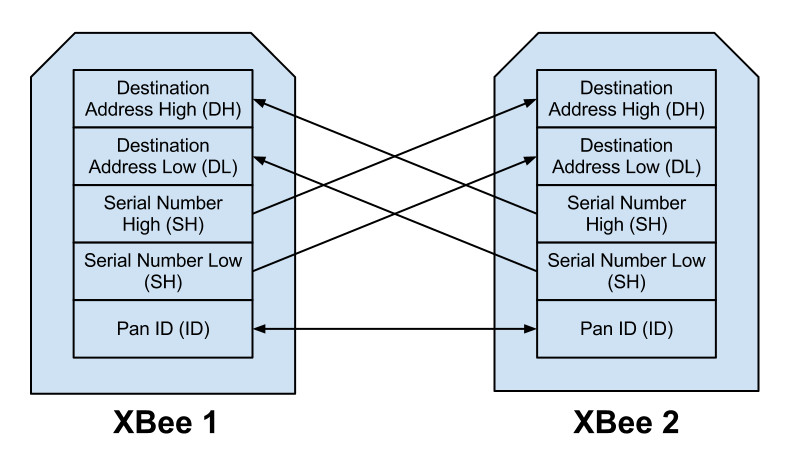
\includegraphics[width=\textwidth]{XBeeDiagram.png}
  \end{column}
\end{columns}
\end{frame}

% ------------------------------------------------------------------
% SLIDE 4 – METHODOLOGY: Telemetry & Ignition Design Decisions
% ------------------------------------------------------------------
\begin{frame}{Methodology — Telemetry \& Ignition Design Decisions}
\begin{columns}[T]
  \begin{column}{0.48\textwidth}
    \textbf{Telemetry — XBee-PRO 900HP selected:}
    \begin{itemize}
      \item 900~MHz ISM band, up to +24~dBm Tx
      \item Link budget at 5~km: \(\text{FSPL} \approx 105.7\)~dB
      \item Received power \(\approx -77.7\)~dBm vs sensitivity \(-110\)~dBm
      \item \alert{Link margin: +32~dB} — robust margin for flight attitude variation
      \item UART transparent mode — direct ESP32 integration
    \end{itemize}
  \end{column}
  \begin{column}{0.48\textwidth}
    \textbf{Ignition — PWM over DC dump:}
    \begin{itemize}
      \item Previous DC dump: burnout in \(\sim\)2~s (single use)
      \item 26~AWG nichrome: \(R = 8.5\,\Omega/\text{m}\)
      \item PWM at 1~kHz with duty-cycle ramp
      \item Target: \(D=0.40\) \(\rightarrow\) \(V_{eff}\approx6\)~V from 15~V bus
      \item \alert{30~s withstand at minimum duty} — confirms controlled thermal approach
      \item IRLZ44N MOSFET: logic-level gate, \(R_{DS(on)}=22\)~m\(\Omega\)
    \end{itemize}
  \end{column}
\end{columns}
\end{frame}

% ------------------------------------------------------------------
% SLIDE 5 – METHODOLOGY: Power Monitoring & Mechanical Design
% ------------------------------------------------------------------
\begin{frame}{Methodology — Monitoring \& Mechanical Design}
\begin{columns}[T]
  \begin{column}{0.48\textwidth}
    \textbf{Power \& Continuity Monitoring:}
    \begin{itemize}
      \item ADS1115 16-bit ADC over I\textsuperscript{2}C
      \item 47~k\(\Omega\)/10~k\(\Omega\) divider scales 14--15~V bus
      \item 14~V \(\rightarrow\) ADC code 19,650 \quad 15~V \(\rightarrow\) 21,060
      \item Clear digital margin for state discrimination
      \item Launch inhibit triggered if battery \(<\)14.0~V or continuity absent
    \end{itemize}
    \vspace{0.3em}
    \includegraphics[width=0.9\textwidth]{{Battery _Monitoring_Proteus_Design.PNG}}
  \end{column}
  \begin{column}{0.48\textwidth}
    \textbf{Mechanical Constraints:}
    \begin{itemize}
      \item 95~mm avionics bay envelope
      \item Four 18650 cells in parallel (4S, 14.8~V)
      \item Dual threaded rods at 50~mm spacing
      \item \alert{Stepped battery-carrier} — edge cells raised to clear rod paths
      \item PETG material for printability and chemical resistance
      \item Upper platform: XBee extension + beacon antenna mounting
    \end{itemize}
    \vspace{0.3em}
    \includegraphics[width=0.85\textwidth]{{FC_Holder Cad.jpeg}}
  \end{column}
\end{columns}
\end{frame}

% ------------------------------------------------------------------
% SLIDE 6 – METHODOLOGY: Software Architecture
% ------------------------------------------------------------------
\begin{frame}{Methodology — Software Architecture (FSM)}
\begin{columns}[T]
  \begin{column}{0.48\textwidth}
    \textbf{FreeRTOS Firmware Modules:}
    \begin{itemize}
      \item Sensor task (GPS, IMU, barometer) @ 10~Hz
      \item Telemetry TX via XBee UART @ 10~Hz
      \item State machine task @ 20~Hz
      \item Deployment channel (event-driven)
      \item ADS1115 monitoring @ 1~Hz
    \end{itemize}
    \vspace{0.4em}
    \textbf{Deployment Arm Conditions:}
    \begin{itemize}
      \item Battery \(>\)14.0~V
      \item Continuity ADC count \(>\)1000
      \item FSM state = APOGEE or RECOVERY
    \end{itemize}
  \end{column}
  \begin{column}{0.50\textwidth}
    \centering
    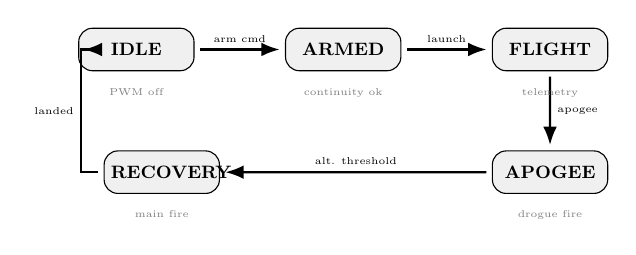
\begin{tikzpicture}[
      >=Latex, scale=0.72, transform shape,
      state/.style={draw, rectangle, rounded corners=5pt, fill=gray!12,
                    minimum width=1.8cm, minimum height=0.75cm,
                    align=center, font=\small\bfseries, text width=1.8cm},
      arr/.style={->, thick, shorten >=2pt, shorten <=2pt}
    ]
      \node[state] (idle)    {IDLE};
      \node[state, right=1.6cm of idle]  (armed)  {ARMED};
      \node[state, right=1.6cm of armed] (flight) {FLIGHT};
      \node[state, below=1.4cm of flight](apogee) {APOGEE};
      \node[state, left=4.8cm of apogee] (rec)    {RECOVERY};
      \draw[arr] (idle)   -- node[above,font=\tiny]{arm cmd} (armed);
      \draw[arr] (armed)  -- node[above,font=\tiny]{launch} (flight);
      \draw[arr] (flight) -- node[right,font=\tiny]{apogee} (apogee);
      \draw[arr] (apogee) -- node[above,font=\tiny]{alt. threshold} (rec);
      \draw[arr] (rec.west) -- ++(-0.4,0) |- node[left,pos=0.25,font=\tiny]{landed} (idle.west);
      \node[font=\tiny, below=0.18cm of idle,  text=gray] {PWM off};
      \node[font=\tiny, below=0.18cm of armed, text=gray] {continuity ok};
      \node[font=\tiny, below=0.18cm of flight,text=gray] {telemetry};
      \node[font=\tiny, below=0.18cm of apogee,text=gray] {drogue fire};
      \node[font=\tiny, below=0.18cm of rec,   text=gray] {main fire};
    \end{tikzpicture}
    \vspace{0.3em}
    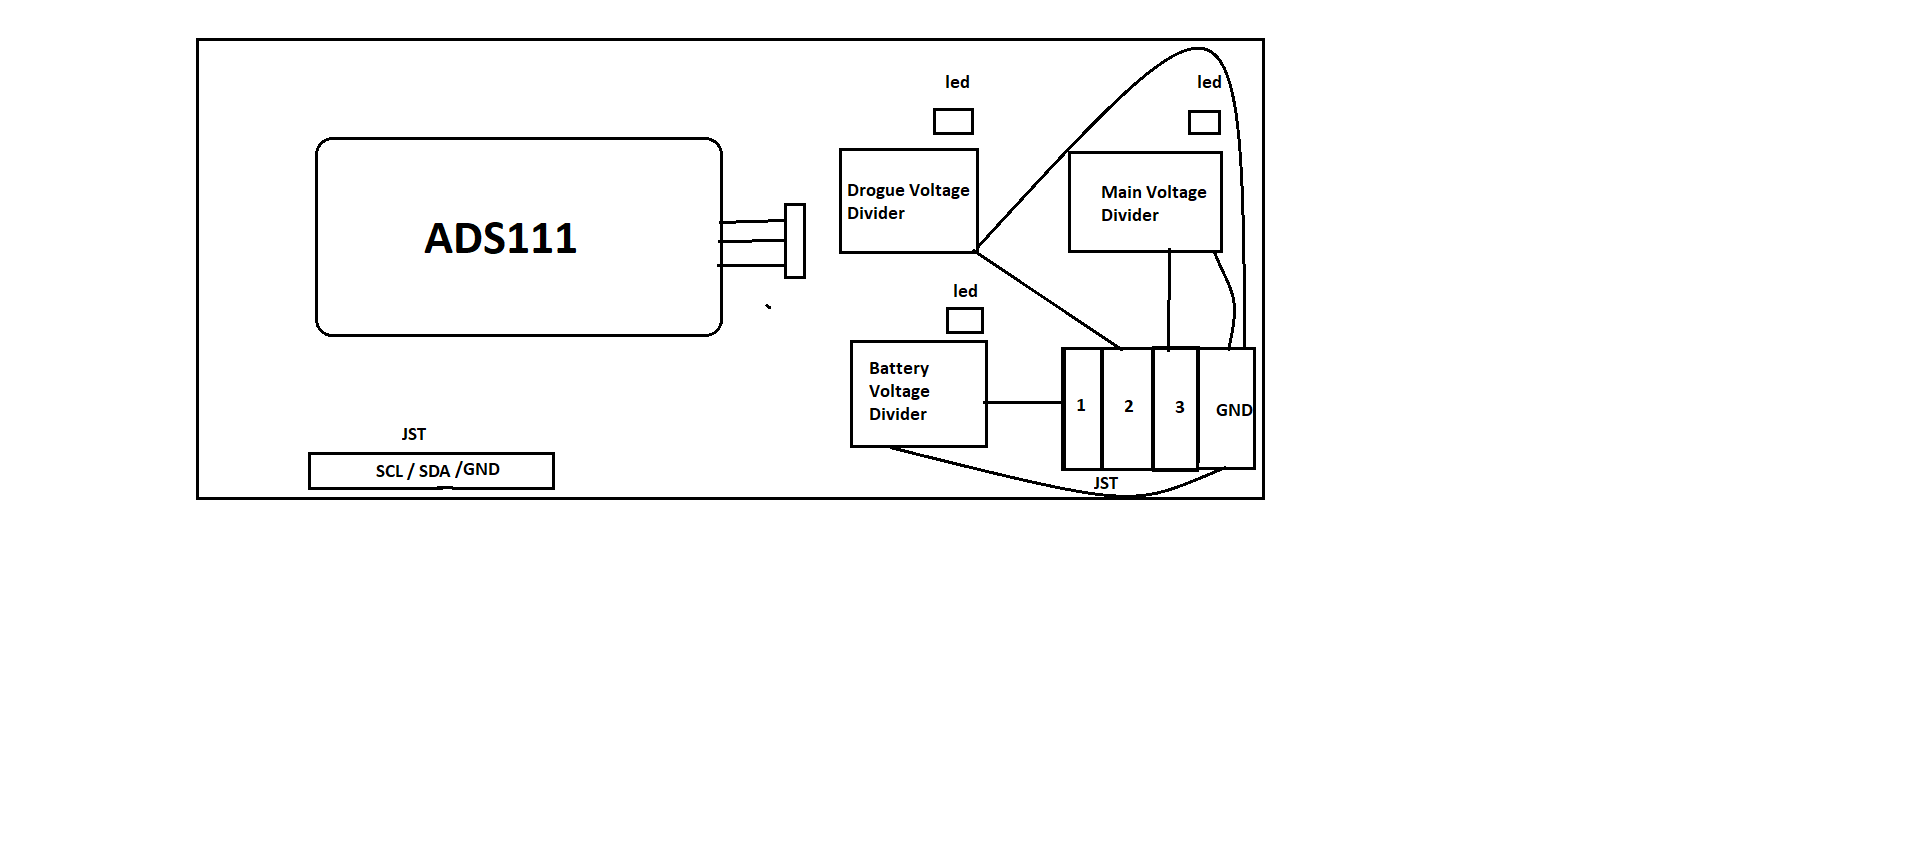
\includegraphics[width=0.9\textwidth]{Power_Monitoring_Design_Concept.png}
  \end{column}
\end{columns}
\end{frame}

% ------------------------------------------------------------------
% SLIDE 7 – METHODOLOGY: Circuit Development Workflow
% ------------------------------------------------------------------
\begin{frame}{Methodology — Circuit Development Workflow}
\begin{columns}[T]
  \begin{column}{0.36\textwidth}
    \textbf{Staged development:}
    \begin{enumerate}
      \item Breadboard wiring validation
      \item Fritzing integration drafting
      \item EasyEDA schematic + PCB capture
      \item Proteus simulation
      \item Bench verification
    \end{enumerate}
    \vspace{0.5em}
    \textbf{Interface strategy:}\\
    UART for XBee (high-rate stream)\\
    I\textsuperscript{2}C for ADS1115 (monitoring)\\
    Segregated pyro / logic routing
  \end{column}
  \begin{column}{0.30\textwidth}
    \centering
    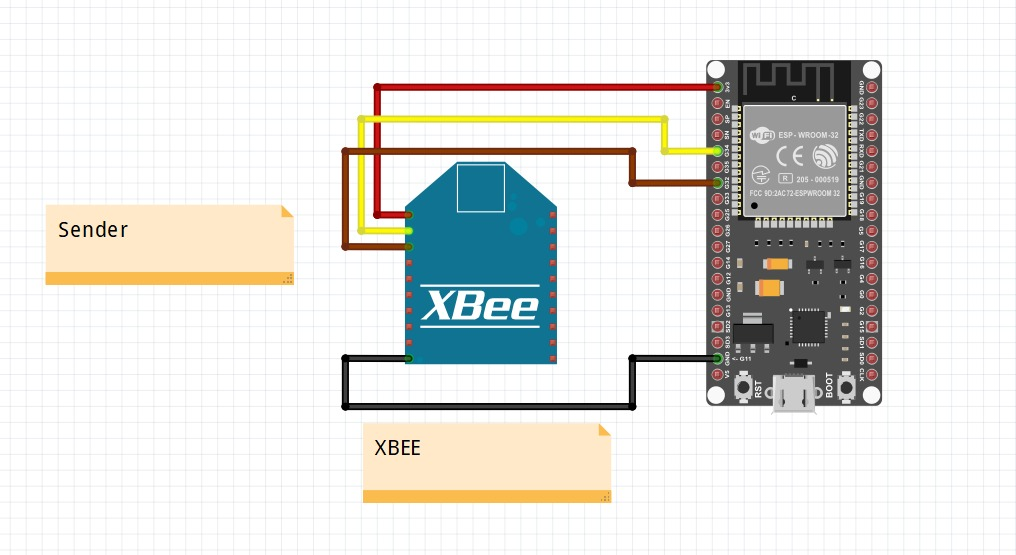
\includegraphics[width=\textwidth]{Rocket_Extension_Design.jpeg}
    \vspace{0.2em}
    {\small Fritzing rocket wiring}
    \vspace{0.5em}
    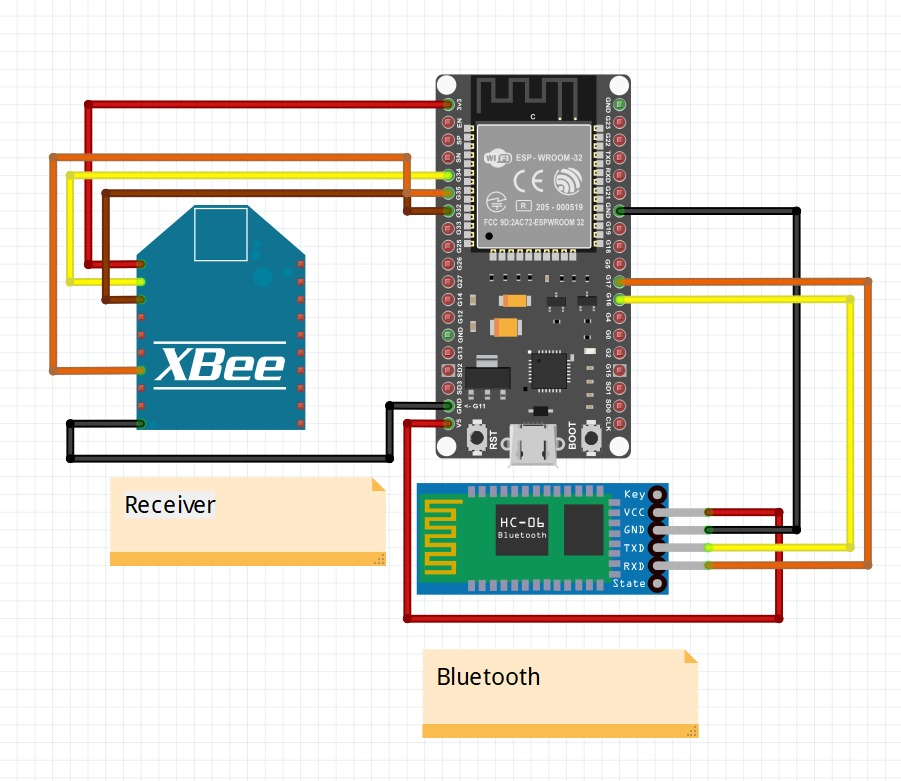
\includegraphics[width=\textwidth]{Base_Station_Design.jpeg}
    \vspace{0.1em}
    {\small Fritzing base station}
  \end{column}
  \begin{column}{0.30\textwidth}
    \centering
    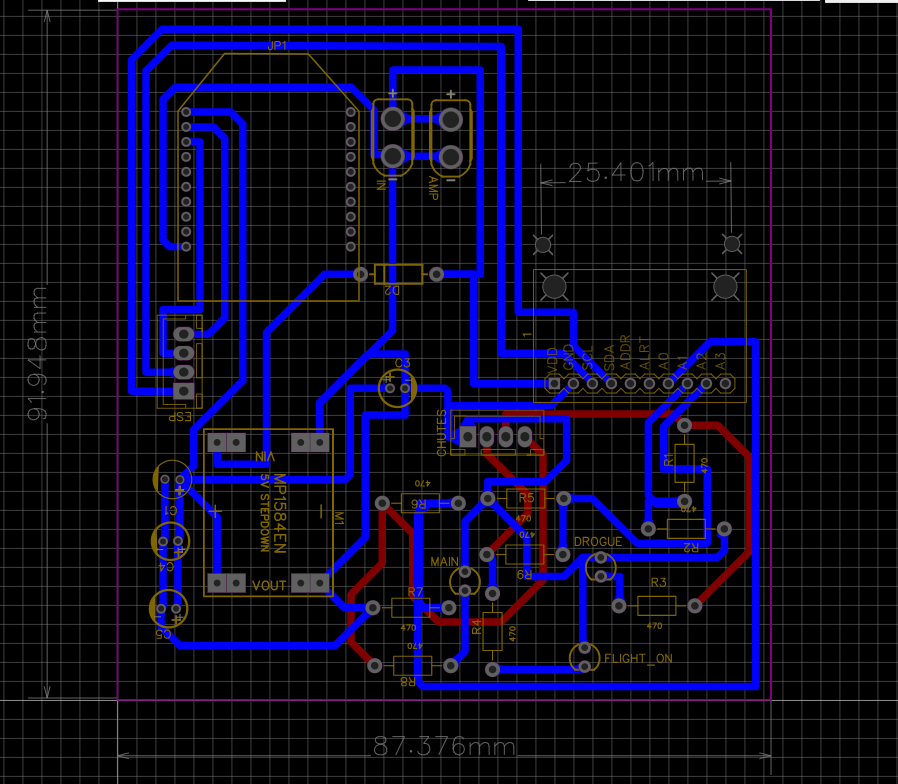
\includegraphics[width=\textwidth]{FC_Xbee_Design__easyDA.PNG}
    \vspace{0.1em}
    {\small EasyEDA schematic}
    \vspace{0.5em}
    \includegraphics[width=\textwidth]{{etched FC circuit.jpeg}}
    \vspace{0.1em}
    {\small Fabricated PCB}
  \end{column}
\end{columns}
\end{frame}

% ------------------------------------------------------------------
% SLIDE 8 – RESULTS: Mechanical Design Outputs
% ------------------------------------------------------------------
\begin{frame}{Results — Mechanical Design Outputs}
\begin{columns}[T]
  \begin{column}{0.33\textwidth}
    \centering
    \includegraphics[width=0.9\textwidth]{{18650_case_cover_without title block.JPG}}\\[2pt]
    {\small 18650 case cover}\\[4pt]
    \includegraphics[width=0.9\textwidth]{{Edge_batt_without title block.JPG}}\\[2pt]
    {\small Edge battery carrier (raised)}
  \end{column}
  \begin{column}{0.33\textwidth}
    \centering
    \includegraphics[width=0.9\textwidth]{{Threaded_Rod_Integration_showing raised battery cells to give way to threaded rods.PNG}}\\[2pt]
    {\small Threaded rod integration}\\[4pt]
    \includegraphics[width=0.9\textwidth]{{Cross_sectional view of avionics bay .jpeg}}\\[2pt]
    {\small Cross-section view}
  \end{column}
  \begin{column}{0.31\textwidth}
    \centering
    \includegraphics[width=0.9\textwidth]{{Avionics assembly.jpeg}}\\[2pt]
    {\small Avionics bay assembly}\\[4pt]
    \includegraphics[width=0.9\textwidth]{{Full Integration in avionics bay.jpeg}}\\[2pt]
    {\small Full integration in airframe}
  \end{column}
\end{columns}
\end{frame}

% ------------------------------------------------------------------
% SLIDE 9 – RESULTS: Electrical Design Outputs
% ------------------------------------------------------------------
\begin{frame}{Results — Electrical Design Outputs}
\begin{columns}[T]
  \begin{column}{0.50\textwidth}
    \textbf{PCB Fabrication (Custom):}
    \begin{itemize}
      \item 65~mm \(\times\) 65~mm, 2-layer FR-4
      \item ESP32 DevKit, XBee UART interface
      \item 2× IRLZ44N MOSFET ignition channels
      \item ADS1115 monitoring circuit
      \item Chemical etching complete
    \end{itemize}
    \vspace{0.3em}
    \includegraphics[width=0.80\textwidth]{{etched FC circuit.jpeg}}
  \end{column}
  \begin{column}{0.48\textwidth}
    \textbf{Proteus BMS Simulation:}\\
    Simulated ADS1115 divider network before PCB bring-up:
    \begin{itemize}
      \item 14~V \(\rightarrow\) \(V_{ADC} = 2.456\)~V (code 19,650)
      \item 15~V \(\rightarrow\) \(V_{ADC} = 2.632\)~V (code 21,060)
      \item Distinct codes confirm reliable state discrimination
    \end{itemize}
    \vspace{0.3em}
    \includegraphics[width=0.95\textwidth]{{Battery _Monitoring_Proteus_Design.PNG}}
  \end{column}
\end{columns}
\end{frame}

% ------------------------------------------------------------------
% SLIDE 10 – RESULTS: Assembled Hardware & Firmware Status
% ------------------------------------------------------------------
\begin{frame}{Results — Assembled Hardware \& Firmware Status}
\begin{columns}[T]
  \begin{column}{0.50\textwidth}
    \centering
    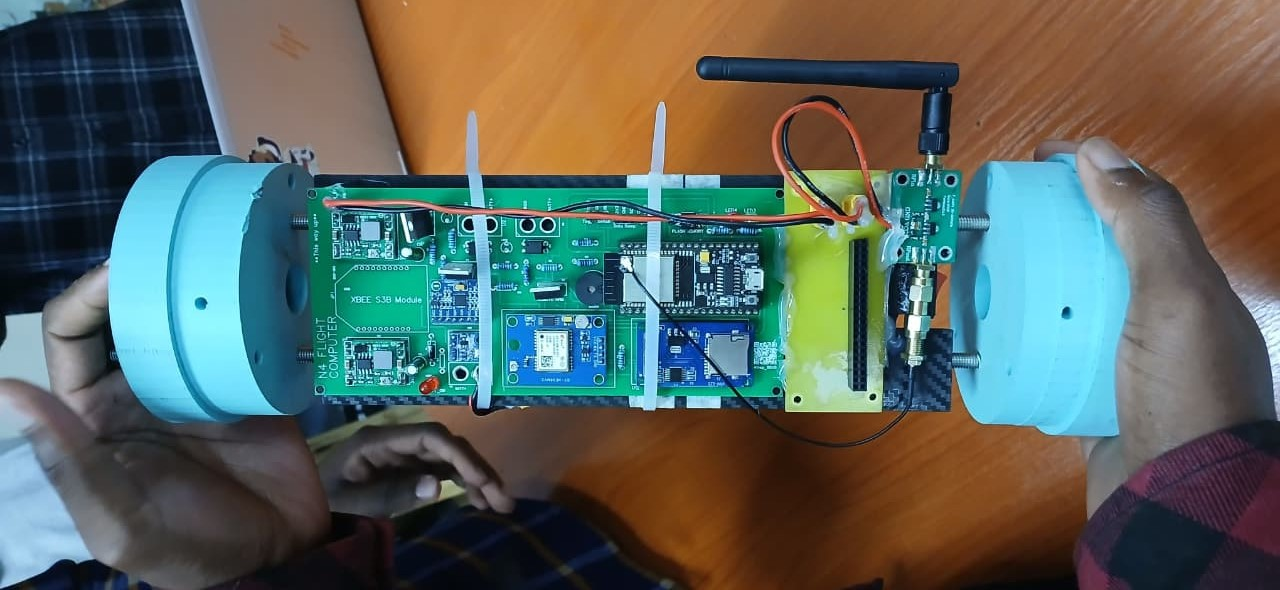
\includegraphics[width=0.85\textwidth]{Assembled_Avionics_Bay.jpeg}\\
    {\small Assembled avionics bay}
  \end{column}
  \begin{column}{0.47\textwidth}
    \textbf{Firmware modules complete:}
    \begin{itemize}
      \item[\(\checkmark\)] XBee UART telemetry (10~Hz)
      \item[\(\checkmark\)] GPS NMEA parsing
      \item[\(\checkmark\)] IMU (MPU6050) \& barometer (BMP280)
      \item[\(\checkmark\)] ADS1115 voltage + continuity monitoring
      \item[\(\checkmark\)] PWM ignition channel with duty ramp
      \item[\(\checkmark\)] Flight state machine (IDLE→ARMED→FLIGHT→APOGEE→RECOVERY)
      \item[\(\checkmark\)] FreeRTOS task scheduler
    \end{itemize}
    \vspace{0.3em}
    \textbf{XBee configured via XCTU:}\\
    Network ID, baud 115200, max Tx power, transparent mode
  \end{column}
\end{columns}
\end{frame}

% ------------------------------------------------------------------
% SLIDE 11 – PENDING WORK
% ------------------------------------------------------------------
\begin{frame}{Pending Design \& Validation Work}
\begin{columns}[T]
  \begin{column}{0.52\textwidth}
    \begin{block}{Hardware Pending}
      \begin{itemize}
        \item PCB population and component soldering
        \item 3D-printed structural parts (PETG) — in production
        \item Aluminium explosion cap holders — pending stock
        \item Full avionics bay integration and fitment check
      \end{itemize}
    \end{block}
    \vspace{0.4em}
    \begin{block}{Testing Pending}
      \begin{itemize}
        \item Open-field XBee range test (0.5–5~km, packet-loss measurement)
        \item ADS1115 voltage accuracy calibration vs reference
        \item Continuity circuit validation with known-R igniter stubs
        \item \alert{Pyrotechnic ignition and pop tests} (pending hardware)
      \end{itemize}
    \end{block}
  \end{column}
  \begin{column}{0.44\textwidth}
    \begin{block}{Firmware Pending}
      \begin{itemize}
        \item Hardware-in-the-loop FSM validation
        \item SD card data logging module
        \item Ground-station command software interface
      \end{itemize}
    \end{block}
    \vspace{0.4em}
    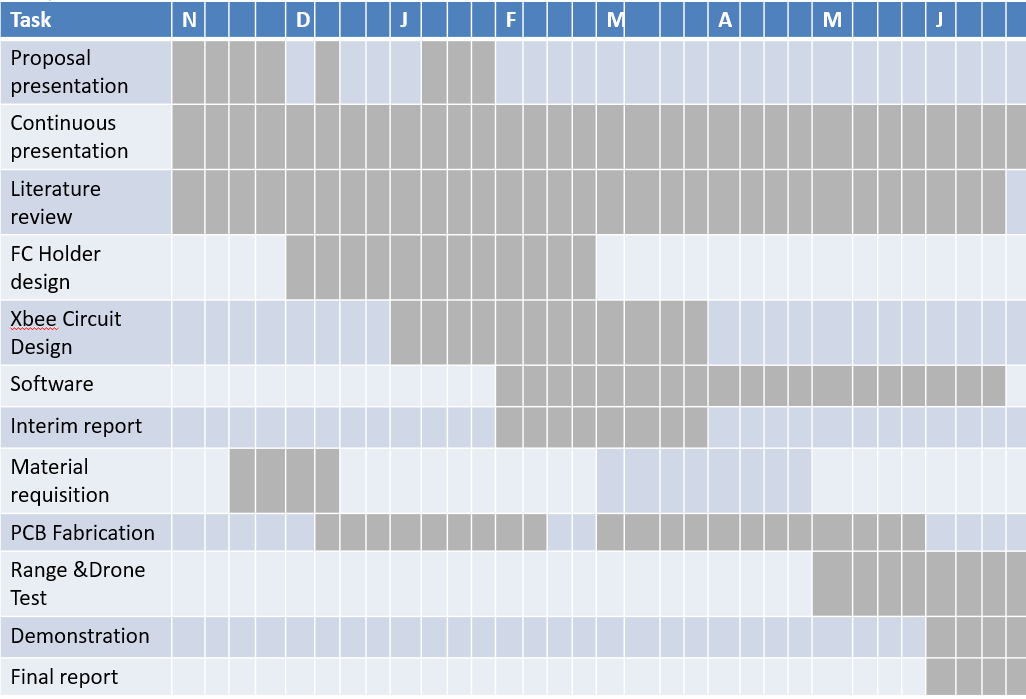
\includegraphics[width=\textwidth]{Timeplan.PNG}\\
    {\small\centering Project Gantt chart}
  \end{column}
\end{columns}
\end{frame}

% ------------------------------------------------------------------
% CLOSING
% ------------------------------------------------------------------
\begin{frame}[standout]
  Thank you\\[0.5em]
  {\normalsize Questions?}
\end{frame}

\end{document}
